\section{Out of vocabulary words}
\begin{frame}{}
    \LARGE N-gram Models: \textbf{Out of vocabulary words}
\end{frame}

\begin{frame}{Out of Vocabulary (OOV) Words}
    \textbf{Problem:} Many words in a language are not present in the training corpus, leading to OOV issues. \\
    \vspace{1em}
    \pause
    \textbf{Example:} The word "quokka" might not be in the training data. \\
    \vspace{1em}
    \pause
    \textbf{Impact:} OOV words can lead to poor model performance and inaccurate predictions. \\
    \vspace{1em}
    \pause
    \textbf{Closed vs. Open Vocabularies:}
    \begin{itemize}
        \item \textbf{Closed vocabulary:} Only words seen during training are recognized.
        \item \textbf{Open vocabulary:} Model can handle unseen words.
    \end{itemize} \\
    \vspace{0.5em}
    \pause
    \textbf{Solution:} Use a special tag \textbf{\texttt{<UNK>}} in the corpus and input to represent unknown words.
\end{frame}

\begin{frame}{Using \texttt{<UNK>} Tokens}
    \textbf{Using \texttt{<UNK>}:} Replace rare or unseen words with the special token \texttt{<UNK>}. \\
    \vspace{1em}
    \pause
    \textbf{Why?} Helps the model generalize to words it has not seen during training. \\
    \vspace{1em}
    \pause
    \textbf{Example:}
    \begin{itemize}
        \item Original: \texttt{I love ChatGPT}
        \item With OOV handling: \texttt{I love <UNK>}
    \end{itemize}
\end{frame}

\begin{frame}{How to Use \texttt{<UNK>} in the Corpus}
    \begin{enumerate}
        \item \textbf{Create vocabulary $V$:} Build a list of all words to be recognized (e.g., most frequent words).
        \item \textbf{Replace OOV words:} For any word in the corpus not in $V$, replace it with \texttt{<UNK>}.
        \item \textbf{Estimate probabilities:} Treat \texttt{<UNK>} as a regular word when computing word probabilities.
    \end{enumerate}
    \vspace{1em}
    This approach allows the model to handle unseen words gracefully during inference.
\end{frame}

\begin{frame}{Example}
    \begin{figure}
        \centering
        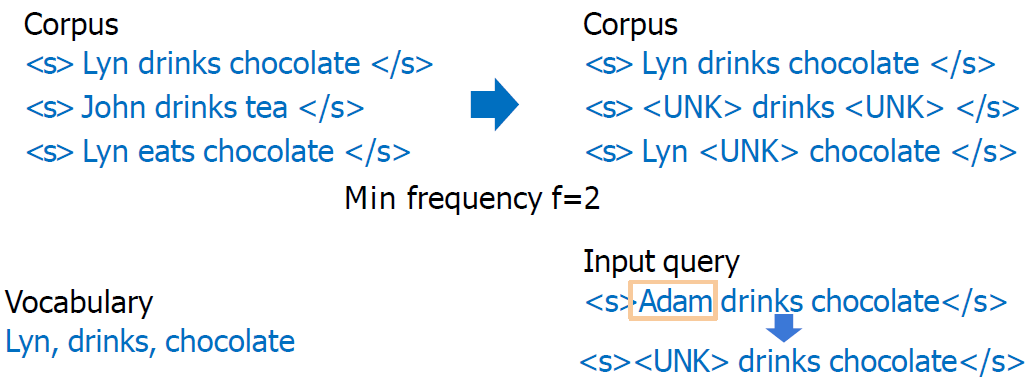
\includegraphics[width=\textwidth,height=0.8\textheight,keepaspectratio]{images/nlp-intro/oov-unk.png}
    \end{figure}
\end{frame}

\begin{frame}{How to Create Vocabulary $V$}
    \textbf{Criteria for Vocabulary Selection:}
    \begin{itemize}
        \item \textbf{Minimum word frequency $f$:} Only include words that appear at least $f$ times in the corpus.
        \item \textbf{Maximum vocabulary size $|V|$:} Limit $V$ to the top $|V|$ most frequent words.
    \end{itemize}
    \vspace{1em}
    \textbf{Use \texttt{<UNK>} Sparingly:} Choose $f$ and $|V|$ to minimize the number of words replaced by \texttt{<UNK>}, while keeping the vocabulary manageable.
    \vspace{1em}
    \textbf{Perplexity:} Only compare language models that use the same vocabulary $V$ to ensure fair evaluation.
\end{frame}